\documentclass[11pt,]{article}
\usepackage[left=1in,top=1in,right=1in,bottom=1in]{geometry}
\newcommand*{\authorfont}{\fontfamily{phv}\selectfont}
\usepackage[]{mathpazo}


  \usepackage[T1]{fontenc}
  \usepackage[utf8]{inputenc}



\usepackage{abstract}
\renewcommand{\abstractname}{}    % clear the title
\renewcommand{\absnamepos}{empty} % originally center

\renewenvironment{abstract}
 {{%
    \setlength{\leftmargin}{0mm}
    \setlength{\rightmargin}{\leftmargin}%
  }%
  \relax}
 {\endlist}

\makeatletter
\def\@maketitle{%
  \newpage
%  \null
%  \vskip 2em%
%  \begin{center}%
  \let \footnote \thanks
    {\fontsize{18}{20}\selectfont\raggedright  \setlength{\parindent}{0pt} \@title \par}%
}
%\fi
\makeatother




\setcounter{secnumdepth}{3}

\usepackage{longtable,booktabs}

\usepackage{graphicx,grffile}
\makeatletter
\def\maxwidth{\ifdim\Gin@nat@width>\linewidth\linewidth\else\Gin@nat@width\fi}
\def\maxheight{\ifdim\Gin@nat@height>\textheight\textheight\else\Gin@nat@height\fi}
\makeatother
% Scale images if necessary, so that they will not overflow the page
% margins by default, and it is still possible to overwrite the defaults
% using explicit options in \includegraphics[width, height, ...]{}
\setkeys{Gin}{width=\maxwidth,height=\maxheight,keepaspectratio}

\title{Estudio ecológico de la familia Malvacease  }



\author{\Large Carolain Pérez Ureña\vspace{0.05in} \newline\normalsize\emph{Estudiante, Universidad Autónoma de Santo Domingo (UASD)}  }


\date{}

\usepackage{titlesec}

\titleformat*{\section}{\normalsize\bfseries}
\titleformat*{\subsection}{\normalsize\itshape}
\titleformat*{\subsubsection}{\normalsize\itshape}
\titleformat*{\paragraph}{\normalsize\itshape}
\titleformat*{\subparagraph}{\normalsize\itshape}

\titlespacing{\section}
{0pt}{36pt}{0pt}
\titlespacing{\subsection}
{0pt}{36pt}{0pt}
\titlespacing{\subsubsection}
{0pt}{36pt}{0pt}





\newtheorem{hypothesis}{Hypothesis}
\usepackage{setspace}

\makeatletter
\@ifpackageloaded{hyperref}{}{%
\ifxetex
  \PassOptionsToPackage{hyphens}{url}\usepackage[setpagesize=false, % page size defined by xetex
              unicode=false, % unicode breaks when used with xetex
              xetex]{hyperref}
\else
  \PassOptionsToPackage{hyphens}{url}\usepackage[unicode=true]{hyperref}
\fi
}

\@ifpackageloaded{color}{
    \PassOptionsToPackage{usenames,dvipsnames}{color}
}{%
    \usepackage[usenames,dvipsnames]{color}
}
\makeatother
\hypersetup{breaklinks=true,
            bookmarks=true,
            pdfauthor={Carolain Pérez Ureña (Estudiante, Universidad Autónoma de Santo Domingo (UASD))},
             pdfkeywords = {palabra clave 1, palabra clave 2},  
            pdftitle={Estudio ecológico de la familia Malvacease},
            colorlinks=true,
            citecolor=blue,
            urlcolor=blue,
            linkcolor=magenta,
            pdfborder={0 0 0}}
\urlstyle{same}  % don't use monospace font for urls

% set default figure placement to htbp
\makeatletter
\def\fps@figure{htbp}
\makeatother

\usepackage{pdflscape} \newcommand{\blandscape}{\begin{landscape}}
\newcommand{\elandscape}{\end{landscape}} \usepackage{float}
\floatplacement{figure}{H}
\newcommand{\beginsupplement}{ \setcounter{table}{0} \renewcommand{\thetable}{S\arabic{table}} \setcounter{figure}{0} \renewcommand{\thefigure}{S\arabic{figure}} }


% add tightlist ----------
\providecommand{\tightlist}{%
\setlength{\itemsep}{0pt}\setlength{\parskip}{0pt}}

\begin{document}
	
% \pagenumbering{arabic}% resets `page` counter to 1 
%
% \maketitle

{% \usefont{T1}{pnc}{m}{n}
\setlength{\parindent}{0pt}
\thispagestyle{plain}
{\fontsize{18}{20}\selectfont\raggedright 
\maketitle  % title \par  

}

{
   \vskip 13.5pt\relax \normalsize\fontsize{11}{12} 
\textbf{\authorfont Carolain Pérez Ureña} \hskip 15pt \emph{\small Estudiante, Universidad Autónoma de Santo Domingo (UASD)}   

}

}






\vskip 6.5pt


\noindent  \section{Introducción}\label{introducciuxf3n}

Este estudio se centra en la Isla Barro Colorado ``BCI'' localizada en
el lago Gatún del canal de panamá. Es un área natural protegida dedicada
al estudio de bosques tropicales y desde su creación ha sido usada como
centro de investigación util para hacer proyectos de investigación.

La vegetación de la Isla Barro Colorado es de bosque tropical húmedo
semi-perenne, propio de climas húmedos tropicales. La mitad de la isla
se encuentra cubierta de bosque jóven de 100 o más años de edad, el
resto está cubierto de bosque viejo, el cual ha sufrido muy pocas
perturbaciones en los últimos 400 años \{moreno2012ambito\}. Se
caracteriza un promedio anual de temperatura de 27\(^{\circ}\) C en
áreas abiertas, con una variación diurna de 9\(^{\circ}\) C. La
precipitación promedio anual es de 2,600 mm, con una estación lluviosa
que va de mayo a diciembre, y una estación seca que comprende los meses
restantes.

Está constituida por un total de 265 especies de plantas, y cada una
pertenece a una familia.La flora es considerablemente más rica en
relación con el tamaño de la isla\{croat1978flora\}.

Dentro de su amplia variedad de familias se encontran las Malvaceae. Es
una planta perteneciente a la familia de las Malvales, con flores
dicotiledóneas, que consta de aproximadamente 244 géneros con
aproximadamente 4225 especies, distribuidas en regiones tropicales a
templadas.

Son plantas de hierbas, arbustos o árboles, generalmente con pelos
estrellados. Los tallos son de fibra de líber robusta con cavidad de
mucílago. Las hojas son simples, alternas, palmadamente divididas,
aserradas, raramente enteras, palmadas veteadas, con estípulas y
pecioladas. Las flores son actinomórficas, solitarias, fasciculadas o
dispuestas en cimas o panículas. A menudo hay epicálices que forman un
involucro alrededor del cáliz, de tres a numerosos lóbulos. Sépalos de 3
a 5, libres o connatos, valvados. Los pétalos son cinco, libres,
giratorios, adnados a la columna estaminal en la base. Los estambres son
numerosos, filamentos connados en tubos, conocidos como adelfos
\{xu2017malvaceae\}.(ver figura 1)

El objetivo de este estudio es analizar como se asocian las especies de
la familia de plantas Malvaceae, y la influencia que tiene los factores
ambientales, del suelo, y geomorfológicos en la distribución de las
especies. Así tambien identificar el conjunto de especie indicadoras,
calcular la distancia Euclidea entre cada especie, medir la asociación,
conocer el método más eficiente para evaluar los datos censales, evaluar
la homogeneidad de sitios, identificar especies indicadoras, calcular
los intervalos de confianza analizar como estan organizados los grupos y
qué patrón presenta en su distribución, así como un análisis de
agrupamiento, estimar, comparar la riqueza de especies y su equidad.
Finalmente integrar ecología numérica para hacer análisis de vencidad y
análisis de autocorrelación.

El lenguaje de programación R La mayor parte del trabajo de modelización
se desarrolló en el entorno de programación, análisis de datos y
producción de gráficos R (R Core Team, 2017). En este entorno
informático, desarrollamos la estrategia de muestreo, el análisis
estadístico, los modelos predictivos, la evaluación de modelos y la
producción gráfica y cartográfica básica. Previamente,

Las preguntas formuladas:

¿Cuál es el método apropiado para calcular la distancia entre especies?
¿Existe una asociación entre las variables ambientales y la distribución
de especies? ¿Existe correlación estadística entre datos de suelo y
composición de especie? ¿Cuáles son los elemntos que debemos buscar para
elegir un método de agrupamiento? ¿Existe una correlación entre las
variables geomorfologicas y

\begin{figure}
\centering
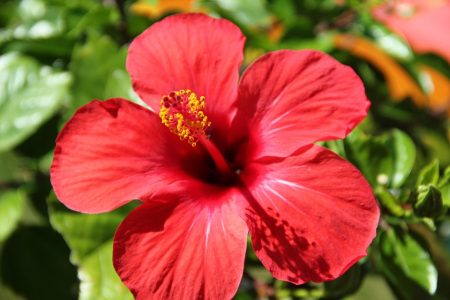
\includegraphics[width=0.40000\textwidth]{Hibiscus-Malvaceae.jpg}
\caption{Figura 1.Flor de la planta Malvaceae}
\end{figure}

\section{Metodología}\label{metodologuxeda}

El estudio se realizó en la Isla de Barro Colorado (IBC), localizada
entre los 9\(^{\circ}\) 09' N y 79\(^{\circ}\) 51' W, que forma parte
del Monumento Natural de Barro Colorado (5,500 ha, Leigh, 1999). Es una
isla formada en 1914, cuando se represó el Río Gatún como parte del
trabajo para la creación del Canal de Panamá \{moreno2012ambito\}. Es
una Zona administrada por el Instituto de Investigaciones Tropicales del
Smithsonian dedicada a investigaciones cientificas.

Dentro de Isla se encuentra la parcela de 50 Hectáreas que tiene 1,000
metros de largo y 500 metros de ancho lo que da un total de 50 ha que se
subdivide en 1 ha. En esta se llevó a cabo nuestro estudio.(ver mapa 1)
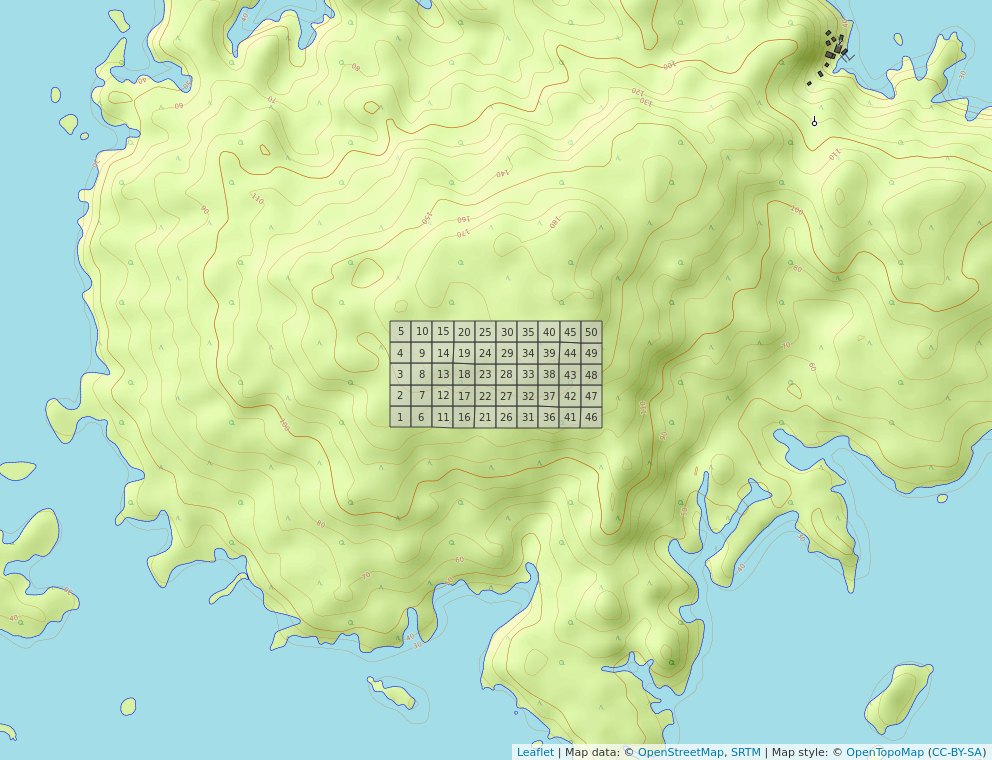
\includegraphics[width=0.60000\textwidth]{mapa_cuadros.png}

En esta primera parte del trabajo se hace un análisis ambiental de
asociación estadística con los datos pre-censales de la parcela de BCI.
Usando una matriz de comunidad convertidas en columnas de hábitats para
generar mapas de abundancia por especie, abundancia de la comunidad,
abundancia de riqueza numérica de toda la comunidad, mapa de simbología
de nitrógeno y simbología del ph.

Se usó la transformación de la matriz de Hellinger, para medir la
asociación de distancia entre sitios; utilizandose la similaridad o la
disimilaridad de Jaccard obteniendose una matriz de distancia de
comunidad transformada a la cuál se le calculó su distancia Euclidea.
Esta distancia Jaccard indica que mientra mayor distancia menor
similaridad, es decir, mientras más crece la distancia el parecido entre
los sitios es cada vez menor.

De este mismo modo para análisis de asociación se usaron las métricas de
modo Q y R; como el coeficiente de correlación de Pearson que mide la
relación estadistica entre dos variables.

La segunda parte del trabajo se basó en el analisis de agrupamiento. Con
el fin de comprobar el método más adecuado se utilizaron los criterio de
enlace simple (se usa distancia mínima), completo (se usa distancia
máxima) y promedio (media entre valores de distancia mínima y máxima,
mejor conocido como UPGM), esto basandos en la matriz de comunidad
transformada a ``normalizada''. Las técnicas elegidas en base a
agrupamiento de manera secuencial, jerarquico por aglomeración,
monotético, aplicando técnicas probabilistacas y no restrigidas. De esto
modo con los valores de abundancia de especie junto con el método de
varianza mínima deagrupamiento de Ward se va construyendo un árbol
dentrítico.

Para efectuar el método más conveniente se usó el criterio de
correlación cofenética, que consiste en la aproximación entre la
distancia cofenética y la matriz de distancias Euclideas a partir de la
matriz de cuerdas. Otro criterio a tomar en cuenta fue la técnica de
anchura de silueta (por el método WARD y UPGMA),que refleja los cortes
del arbol en varios grupos usando la posición que ocupa el promedio más
alto. En este caso el valor de anchura promedio fue 2 con 3 sitios. En
un principio se descartaron los grupos con menos de 3 sitios, sin
embargo el valor máximo más proximo tenian mucha diferencia con el valor
de la posición 2, por lo que se puede decir que la posición 2 es la más
optima.

Para evaluar homogeneidad de promedios usaron las pruebas TStudent
(medias), y la prueba no paramétrica de la suma de rangos de Wilcoxon
(medianas), usando como variable de agrupamiento los grupos establecidos
en el agrupamiento UPGMA y Ward.Estas sirvieron para hacer una
correlación con los resultados de abundancia global y riqueza.

Con el análisis de especies indicadoras mediante Indval se obtuvieron
las especies consideradas como indicadoras y un análisis de especies con
preferencia por hábitat mediante el coeficiente de correlación biserial
puntual. Con la técnica de boostrap multiescalar (BP) se calcularon los
intervalos de confianza también conocidos como valores de probabilidad
insesgada (AU). Dicha técnica consiste en un método de remuestreo de
datos que permite resolver problemas relacionados con la estimación de
intervalos de confianza o la prueba de significación estadística
\{ledesma2008introduccion\} de este modo se usó la prueba de permutación
que se usa para obtener una mayor precisión de resultados.

Con la prueba de ANOVA y Kruskal-Wallis se evaluaron la homogeneidad de
medias y medianas representadas por paneles de diagrama de cajas.

Dentro del análsis de agrupamiento, se realizó la ordenación simple (no
restringida) usando la técnica PCA y la ordenación canónica
(restringida). En el primer caso, las tendencias detectadas en el
conjunto de datos de interés, no están restringidas por otro conjunto.
En el segundo caso, las tendencias detectadas en un conjunto de datos se
asocian a otro conjunto. En la técnica PCA por sus siglas eningles
``principal components analysis'' se usó la variable de suelo a través
para generar del gráfico de escalonamiento.

En los Análisis de diversidad alpha y beta (di) se determinaron dos
componentes principales que fueron la riqueza y equidad. En el análsis
Alpha el indice de la entropia de Shannon se usó para medición el indice
de equidad de Pielu

Otro indice es el de concentración de Simpson es un indice que mide la
concentración. El método de la ralefacciones se usa para poder estimar
combinaciones. Estima una riqueza para las muestras que se dividen en
dos metodos asintóticos y no asintóticos. La entropia de Renyi
generaliza estos 3 indices anteriores y se obtienen los números de
diversidad de Hill.

En el análisis beta se busca la equidad usando la aproximación de
Whittaker, asociada a los números de Hill y la ratio. Y la otra parte
identificar las especie y sitios que contribuyen a la diversidad beta.

Ecología numérica

Se realizaron análisis de vencidad, un análisis de autocorrelación
espacial mediante correlograma de puntos, análisis de correlación a
apartir de multiples variables como abundancia de especies y variables
ambientales usando el resumen estadistico y de correlograma aplicandolo
a la matriz de comunidad. De este modo se aplicaron técnicas del
programa mantel para determinar la correlación entre dos matrices de
distancia y determinar autocorrelación mediante la prueba de permutación
para I de moran,utilizando los denominados lisa ba.

EL analisis de autocorrelación de una variable ambiental en este caso
ph, A traves del metodo I Moran se analizaron la correlación de la
variable PH no se ve autoccorrelación espacial de acuerdo a los
resultados de estimación y expectativa, en el orden 9 la autocorralzión
es positiva y este implica 10 sitios.

\section{Resultados}\label{resultados}

Análisis ambiental

\begin{figure}
\centering
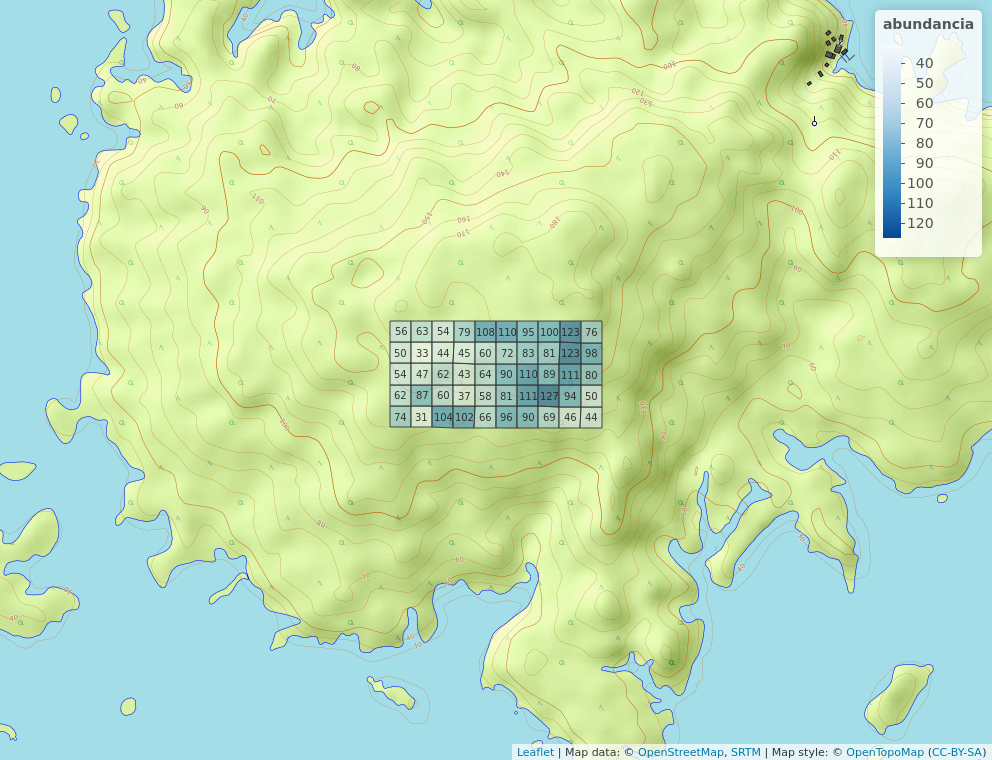
\includegraphics[width=0.50000\textwidth]{mapa_cuadros_abun_mi_familia.png}
\caption{Districución de la abundancia por cuadros de 1 de la familia
Malvaceae Ha}
\end{figure}

La mayor abundancia de la familia Malvaceae se concentra en el cluster
de la parte oriental, mientras que en la parte occidental los cluster
son de baja abundancia.La abundancia global se concentra en la parte
occidental, por lo tanto mi familia no sigue el patron que siguen todas
las plantas de familia de BIC.

\begin{figure}
\centering
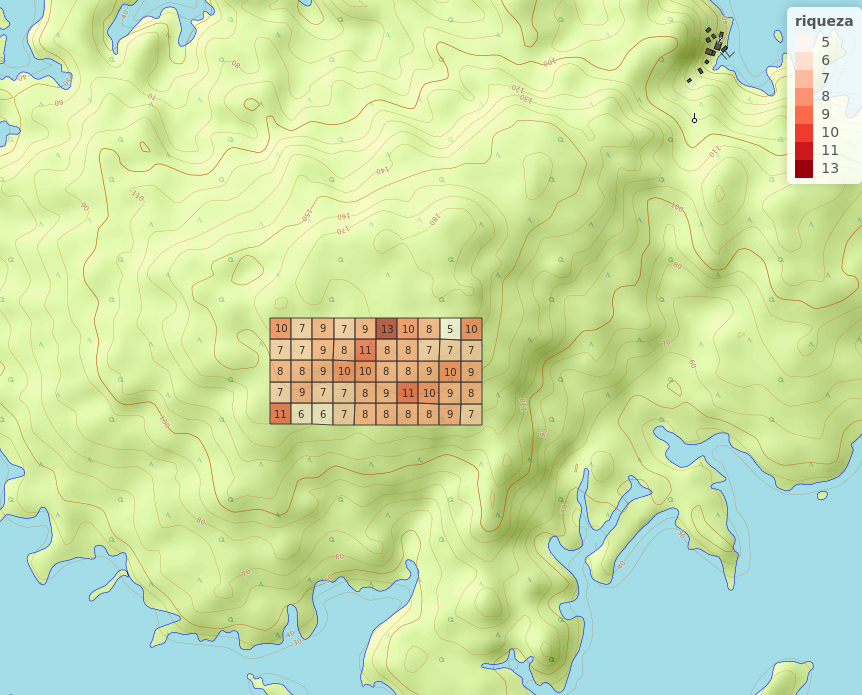
\includegraphics[width=0.50000\textwidth]{mapa_cuadros_riq_mi_familia.png}
\caption{Districución del riquezas por cuadros de 1 Ha}
\end{figure}

Las riquesas máximas en la familia de plantas Malvaceae se encuentran en
el borde superior central, a diferencia de los patrones de riqueza
global que se encuentran en el centro y al borde noriental.

\begin{figure}
\centering
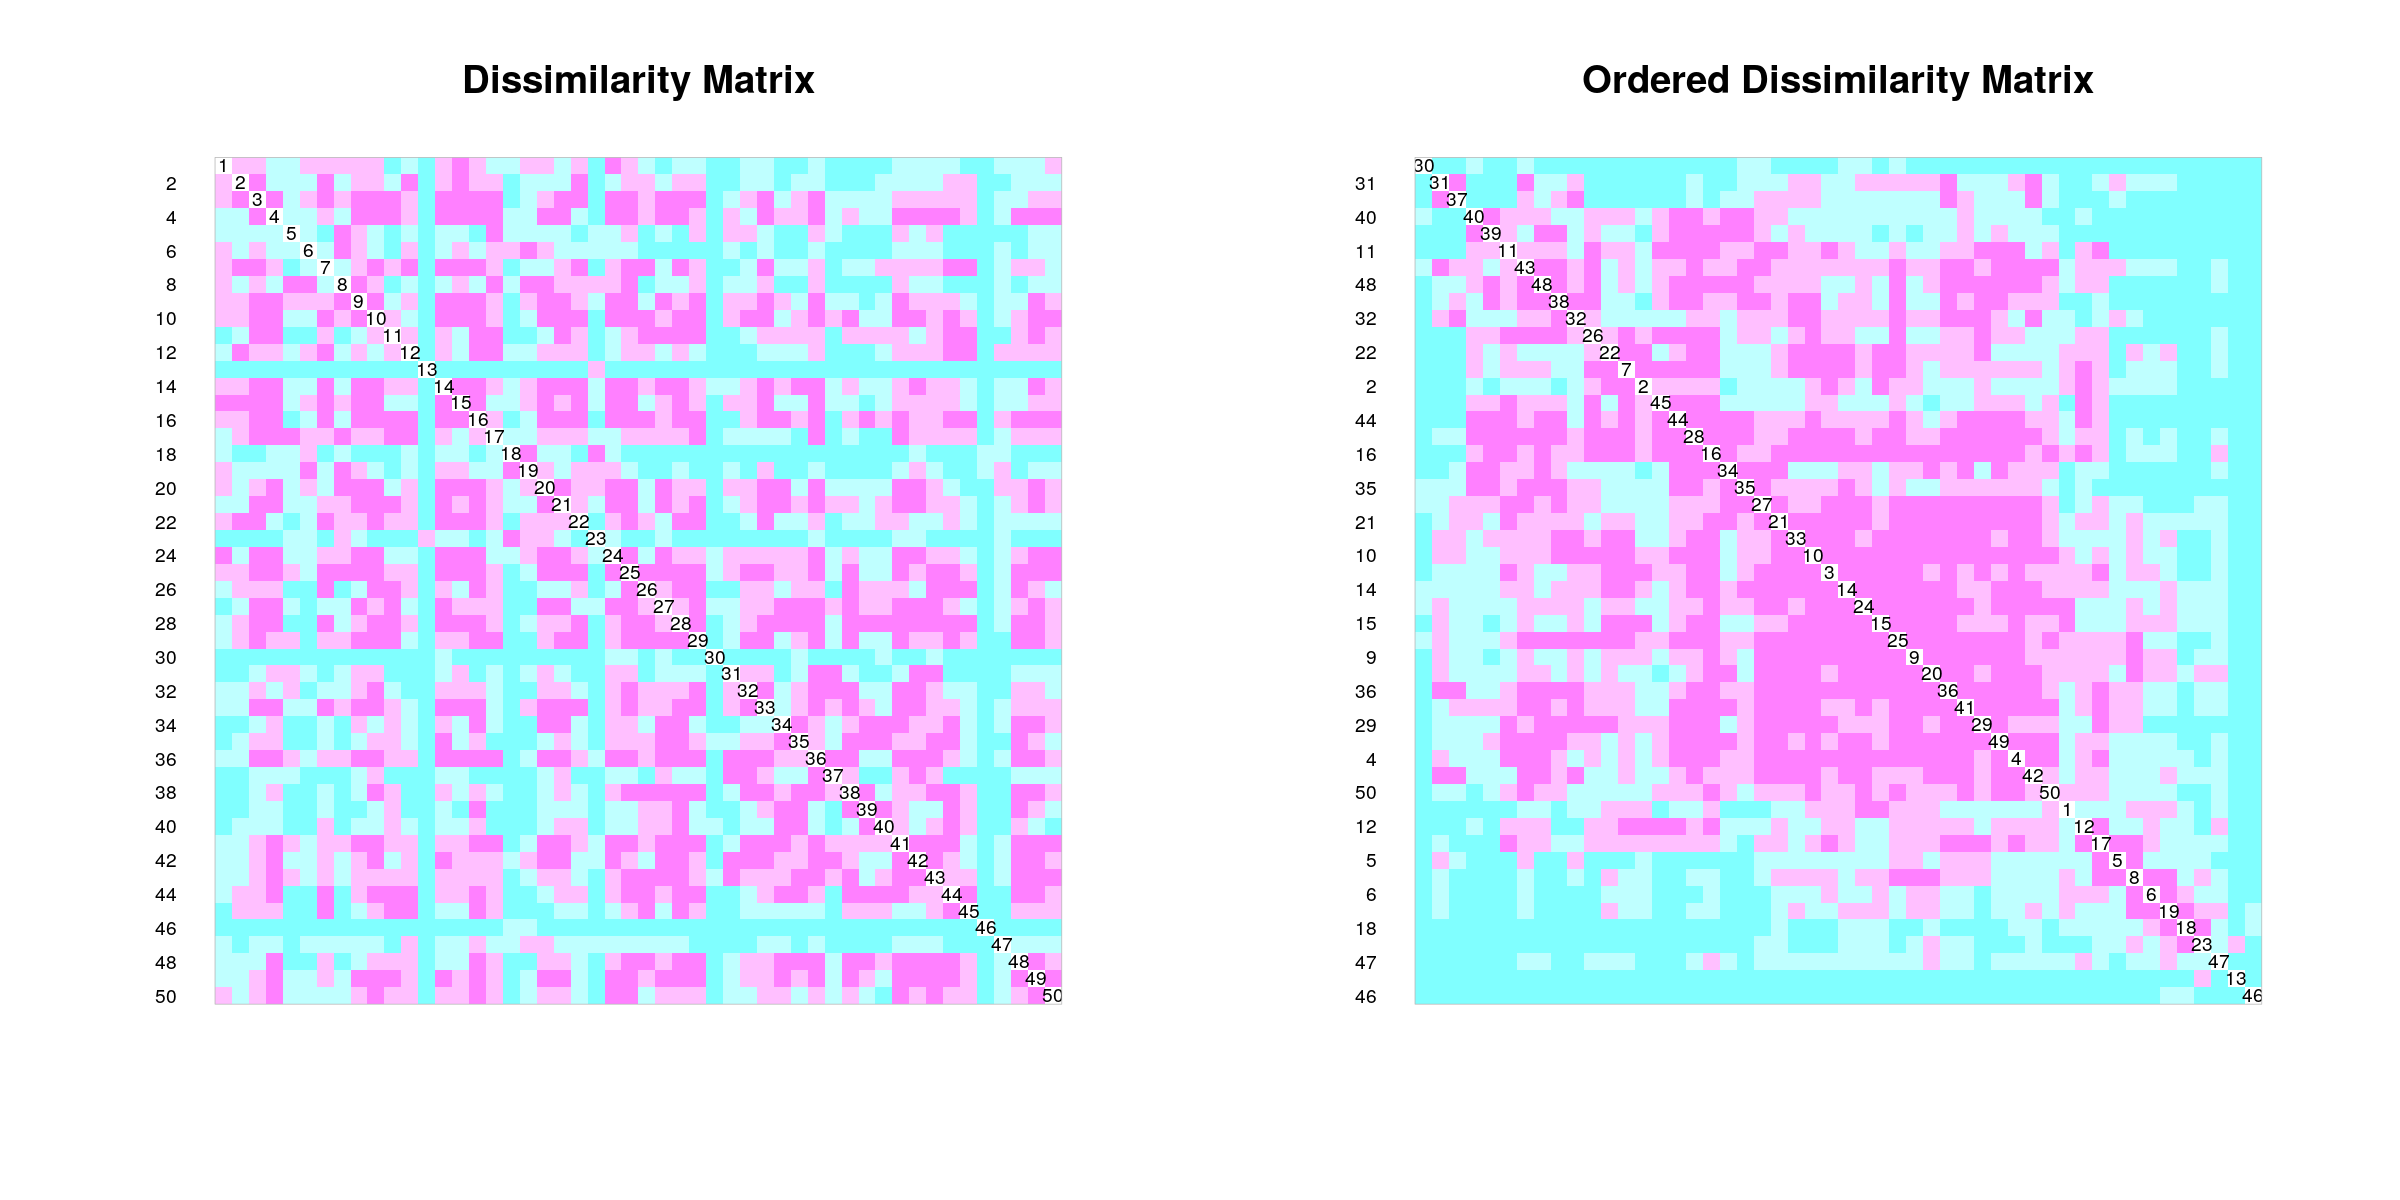
\includegraphics[width=0.50000\textwidth]{matriz_disimilaridad_hellinger.png}
\caption{Matriz de
disimilaridad\label{fig:matriz_disimilaridad_Hellinger}}
\end{figure}

En este mapa de calor se muestran dos matrices de distancia, la primera
ordenada en función del orden que van apareciendo los sitios y la otra
ordenada en función de la fuerza de asosiación Euclidea de la matriz
transformada Hellinger. Los clústers muestran una fuerte asociación
entre los sitios 22 al 50 en el centro, lo que indica estos lugares
tienen una cierta asociación en cuanto a sus espepcies compartidas y
desde el punto de vista de la distancia Jaccard están muy próximos.

recordando el color rosado indica distancia corta y mientras más cortas
los cluster se parecen entre sí.

\begin{figure}
\centering
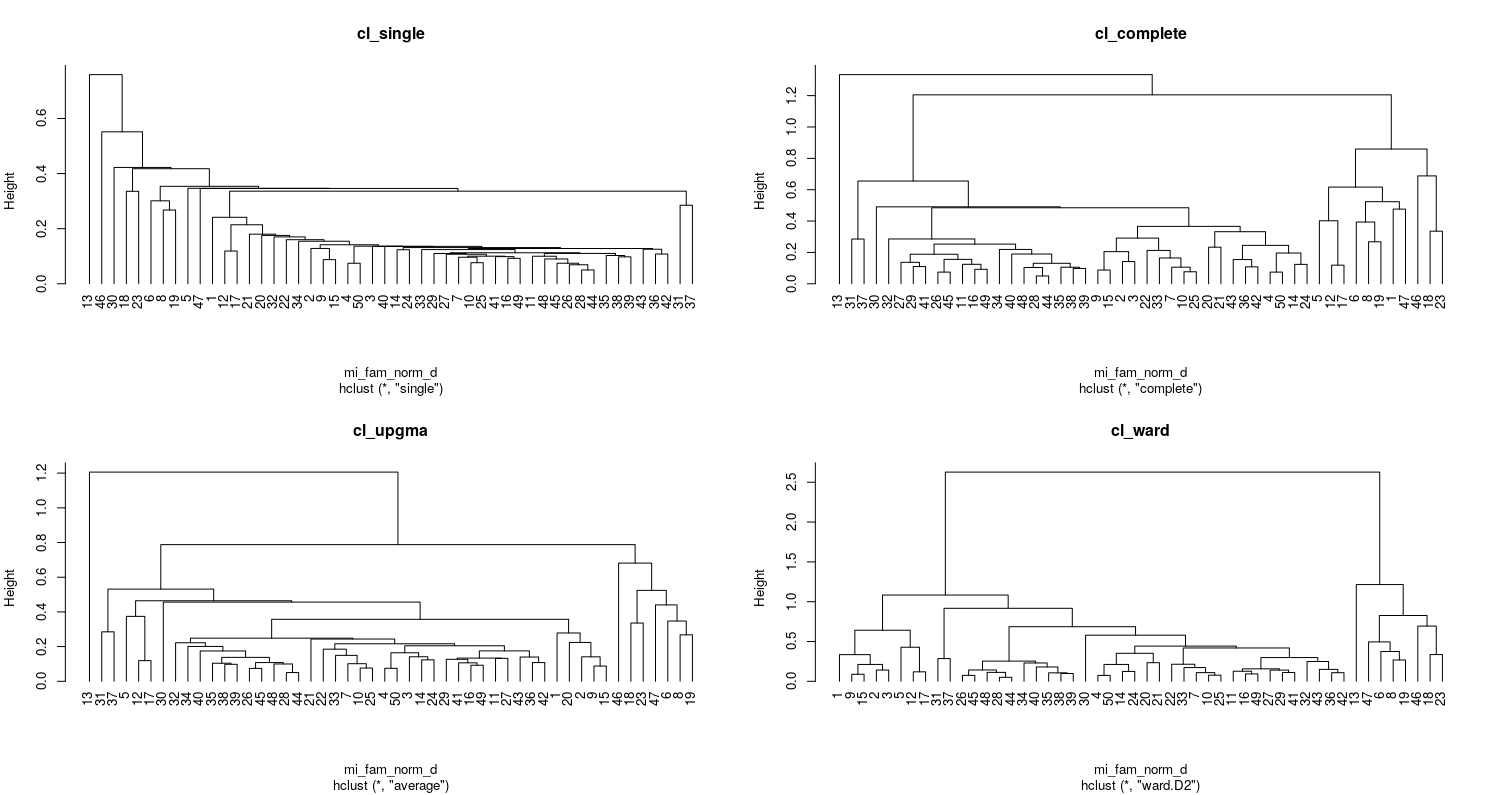
\includegraphics[width=0.50000\textwidth]{4_dendogramas.png}
\caption{Dendogramas por los cuatro métodos}
\end{figure}

Este es el dendograma generado con los métodos de enlaces simple,
completos, UGMA y Ward. Se muestran una distancia diferente entre los
nodos de altura. Los cortes fueron muy desiguales en el método UPGMA,
completo y simple donde se abarcó 2 grupos; en el primer grupo tenía 7
sitios de árboles, otro grupo solo un sitio (el sitio 13), y el 3er
grupo poseía los 42 restantes.(ver figura 2)

Tomando el criterio de la correlación cofenética y el método de anchura
de silueta,se hizo un contraste entre el método UPGMA y WARD. Con el
método UPGMA el promedio de anchura de silueta sugería usar 2 grupos un
grupo grande y otro pequeño, sin embargo aparece un tercero en el mapa
de calor.

El grupo grande ocupa la mancha rosa central que se extiende hasta el
borde inferior derecho, y el grupo pequeño ocupa la posición superior
derecha. (ver figura 3) Aunque los promedios de anchura de siluetas
sugerían usar 2 grupos, el mapa de calor parece sugerir que existe un
tercer grupo entre los dos anteriores, representado por los sitios 18,

Evaluación mediante remuestreo por \emph{bootstrap} multiescalar

No obstante, aun con todas sus bondades, los datos censales carecen de
una fortaleza: no reflejan asociación con grandes unidades de hábitats
y, a lo sumo, revelan asociación con microhábitats muy específicos, por
lo que extraer conclusiones sobre patrones de asociación con variables
ambientales de manera más general, presenta sus limitaciones.

un método que consiste en tomar muestras aleatorias de los datos y
realizar, con cada una, análisis de agrupamiento. Este proceso se repite
varias veces (e.g.~1000 veces), es decir, se realizan varias
iteraciones. Al finalizar, se cuenta la proporción de veces que un grupo
dado aparece consistentemente como clúster (tasa de éxito), la cual se
denomina probabilidad de \emph{bootstrap} del clúster en cuestión
(\emph{bootstrap probability}, BP). A este procedimiento se le ha
añadido más recientemente el criterio de remuestreo por \emph{bootstrap}
multiescalar, es decir, considerar muestras de tamaños diferentes, a lo
que se denomina valores de probabilidad aproximadamente insesgados
(\emph{approximately unbiased}, AU). Los valores de AU son, en
principio, más fiables que los de BP, por lo que serán los preferidos en
este análisis.

Rectángulos de borde azul, para todos aquellos grupos que resulten con
valores de AU\textgreater{}0.91 en sus nodos. Estos rectángulos
permitirán ver los grandes grupos sin perder robustez, dado que prefiero
el enfoque de agrupador (\emph{lumper}) por encima del desglosador
(\emph{splitter}); con esto además evito la tendencia de dividir en
demasiados grupos pequeños, la cual vengo evitando desde análisis
anteriores por el alto grado de autocorrelación espacial que afecta a
los datos de BCI.

En este caso, el valor de anchura promedio de la posición 2 se
diferencia, por mucho, del de la posición 3. Por lo tanto, puedo elegir
con seguridad 2 como número de clústers óptimo.

se dedujo que el metodo mas apropiedo era Ward por ser el mas facil de
entender. Con el método Ward fué más facil de entender, ya que los
cortes

A todo esto se dedujo que fué el método más a apropiado.

\begin{figure}
\centering
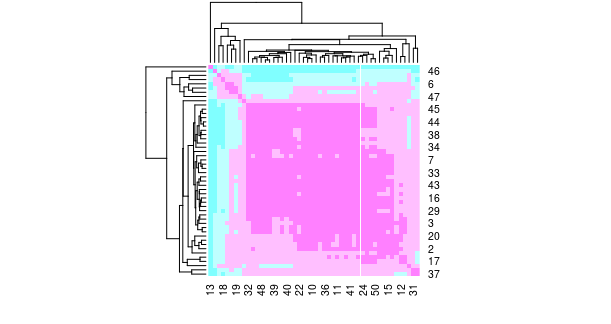
\includegraphics[width=0.50000\textwidth]{anchura_siluetas_matriz.png}
\caption{Matriz anchura de siluetas}
\end{figure}

El siguiente mapa corresponde a un mapa de calor entre el dendorama,
mientras más rosado hace referencia a una aproximación entre sitios y el
azul representa a la lejania que existen entre los sitios.

En el primer grupo de cluster se identifica que los sitios localizados a
su izquierda están muy cercanos pero los que le quedan a su derecha muy
distantes. n este mapa de calor lo que se refleja son las distancia
reflejas de un sitio a otro en cuanto a su composición.

Se relfleja que los primeros clustes represntados por 7 grupos se ven
mas separado del resto. Los 42 sitios restantes forma un cluster enorme
juntos entre sí El sitio 17 quedó como una hoja aislada.

\begin{figure}
\centering
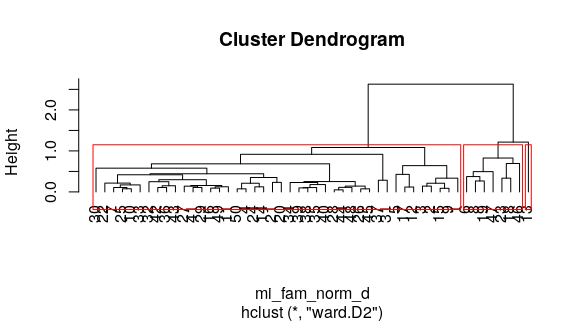
\includegraphics[width=0.50000\textwidth]{cluster_ward.png}
\caption{Dendograma en divididas en 3 grupos por el método ward}
\end{figure}

Figura 2

Se generaron mapas de todas las variables ambientales por medio de
paneles

Cuando se crea la matrix y se crea un panel de correlación mostrando
datos de dos colores, el coeficiente de correlación cuando esta en azul
no es estadisticamente significativa, cuando está en rojo si es
significativa.

se puede encontrar que la organización de las especies por grupos está
influenciada por estas variables cuando las pruebas no son
significativas presentan una mediana mas o menos a la misma altura.

El porcentaje de interfluvios podria estar asociandose por la
composición de especie, es decir,que de acuerdo a la posición
geomorfológica puede encontrarse una determinada especie.

Especies indicadoras (hacer cuadro)

La homogeneidad de promedios se evaluaron mediante las pruebas T de
Student y la suma de rango de Wilcoxon por el métodos de ward divididas
en dos grupos.Las variables B, Mn, N, Ph,P resultaron ser
significativamente diferentes y en el relieve de porcentaje es la
pendiente media (ver figura 3).

De esta forma los valores mas elevados del grupo 1 que son las variables
Mn y N marcan una acidez mayor.
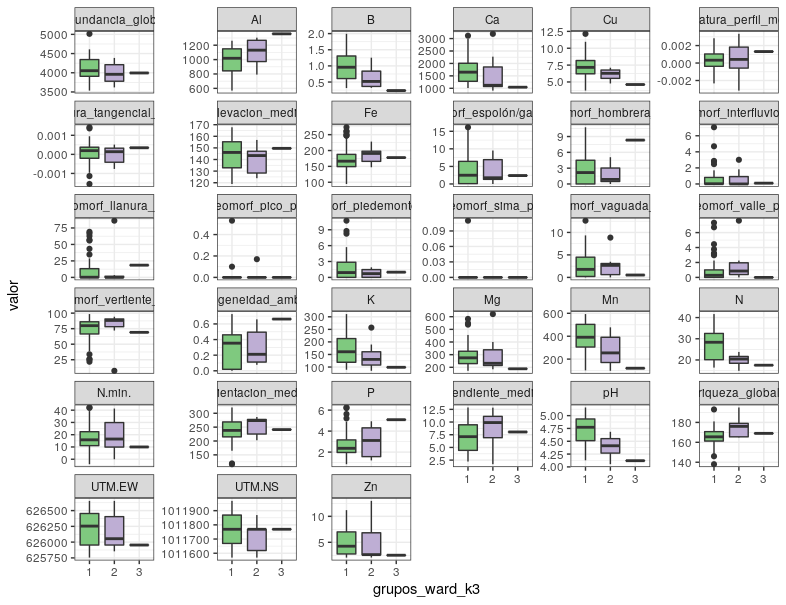
\includegraphics[width=0.70000\textwidth]{variables_ambientales.png}

Las especies indicadoras se obtuvieron mediante el método Indval, se
encontraron en total 3 especies que pueden ser consideradas como
indicadoras. en el grupo 1 se encuentró una 1 especie indicadora, esto
quiere decir que es una especie extremadamente signicativa en la prueba
de permutación.

aa3

Técnicas de ordenación

\begin{figure}
\centering
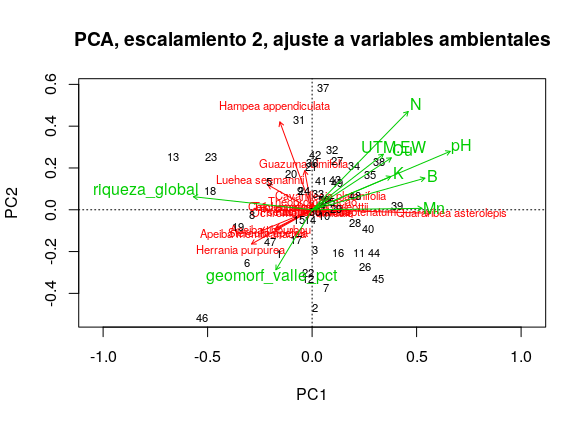
\includegraphics[width=0.50000\textwidth]{Escalonamiento_ajustado_variables_ambientales_PCA.png}
\caption{Biplot Escalonamiento de variables ambientales por el método
PCA}
\end{figure}

Aqui se presentan las variables que resultaron asociadas de acuerdo con
la prueba de permutación, ante un nivel de significacia de 0.05,esto
significa que muchos de los datos asociados de suelo se relacionan con
la matriz de comunidad lo que lo convierte en análisis consistentes. De
acuerdo a la definición se trata de una ordenación no restrigida con
ajuste pasivo. Hay mas autocorrelación hacia el Oeste.Las especies estan
mostradas en color rojo y los elementos en colores verdes.

t02 Las varaianza tanto restringida con no restrigida muestra un valor
de 0.48 y 0.52 l que quiere decir que el suelo es importante.

El valor de varianza insesgado dió como resultado un 0.29,esto explica
es que solo se explica un 29 \% de los componentes del suelo, resulta
ser un valor muy bajo.El grado de preferencia de cada especie la
abundancia de especies por cada sitio está variando y eso es por las
variables del suelo por lo menos en un 29 \%

\begin{figure}
\centering
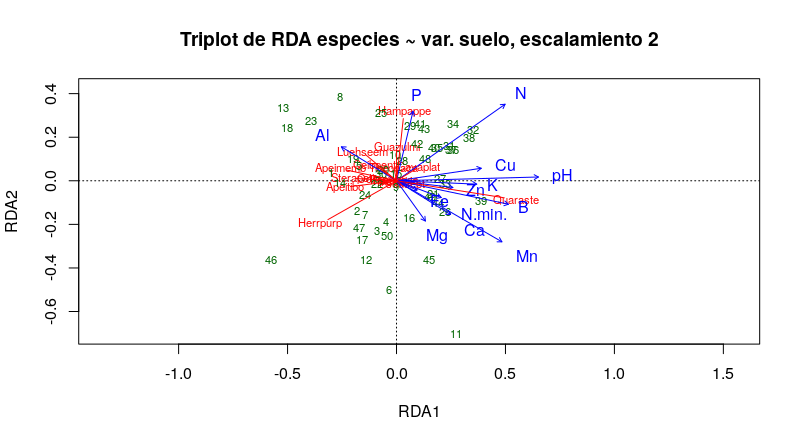
\includegraphics[width=0.50000\textwidth]{triplot_especies_variables.png}
\caption{Triplot de especies y variables de RDA}
\end{figure}

El RDA anterior mostró que las variables de suelo zinc y potasio, al
igual que calcio y magnanesio. Esto es útil para predecir la matriz de
comunidad. Hay mucha colinealidad entre algunas variables.

Se excluyeron algunas variables por no ser significativas como el caso
de B Y Ca y dió como resultado graficos similares ningun vector se
superpone,sitios asociados con las variables de suelo.

Hay una proprocion de varianza sesgada se quitaron las colineales, la
varizanza sesgada es menor que la de matriz ambiental de suelo.En el
triplot las distancias auclidias y entre los siito hacen sentido Se nota
que hay un cluster de sitios en asociada con heterogeneidad ambiental.La
que contribuyen más es la especie que tenga la puntacione mas corta en
este caso viene siendo Guazulmi

El analisis de correspondencia canónica se basa en el ajuste de
distancia ji cuadrado hacia variables ambientales, El particionado de la
distncia ji cuadrado escalada indica caunto estoy consiguiendo explicar
por la via de la ordenación restrigida Las especies raras o excluidas
son Apeitibo" ``Cavaplat'' ``Ceibpent'' Al hacer los datos por el metodo
de distancia de ji cuadrado es muy dificil hacer los analsis La
proporción de ji cuadrado no aumenta se mantuvo igual. En ji cuadrado
escalado insesgado tiene una disminución no tan significante. Al ser
sisitos tan autocorrelacionados no es tan facil hacer un análisis por
los sitios esta agolpados entre sí

\begin{figure}
\centering
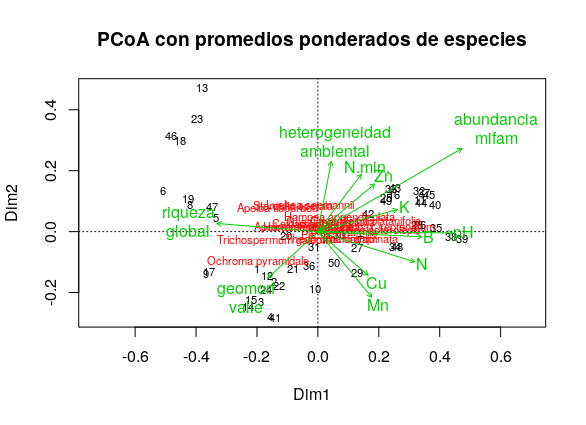
\includegraphics[width=0.50000\textwidth]{metrica_PCoa_con_promedio_ponderado_especies.png}
\caption{Gráfico de promedios ponderados por especies por la métrica
PCA}
\end{figure}

Análisis alpha y beta

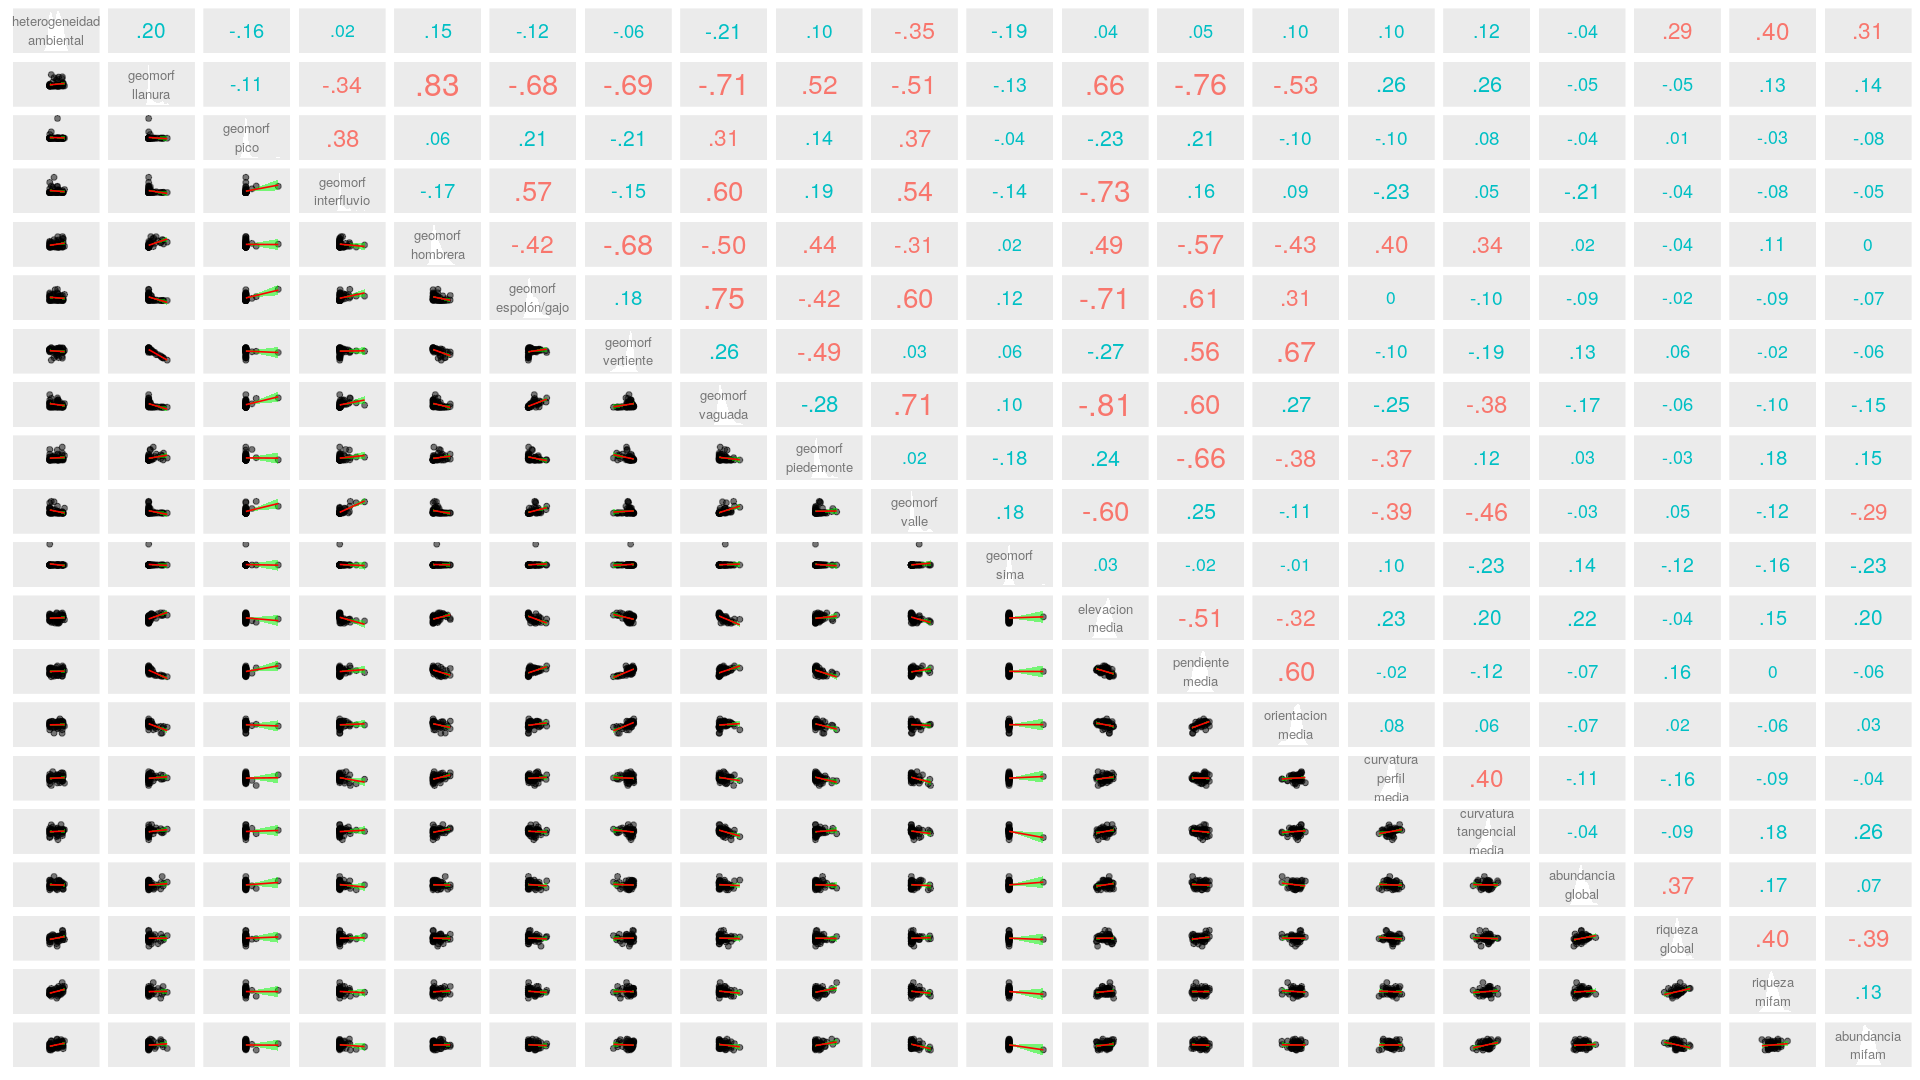
\includegraphics[width=0.50000\textwidth]{matriz_correlacion_geomorf_abun_riq_spearman.png}
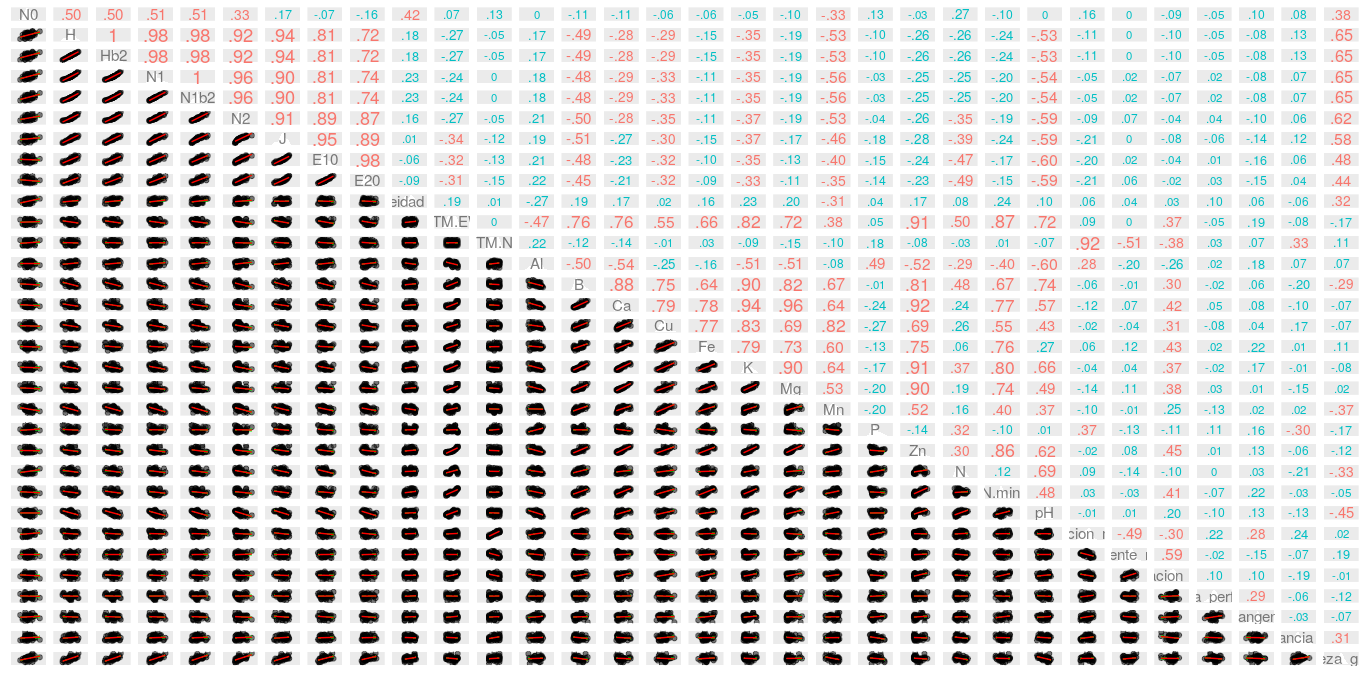
\includegraphics[width=0.50000\textwidth]{Representacion_especies_variables_ambientales.png}

La diversidad alpha

En este panel pocas parte de los elementos (números de entropia y ratios
de hill) han presentado una fuerte asociasion con las variables
geomorfológicas. Sin embargo los mismo muestran una fuerte asociación
con las variables ambientales tales como el boro,calcio,manganesio, y
una correlación altisima con el PH por esta razón es baja en Aluminio.
Podemos concluir que el Ph es la variable de suelo más representativa en
esta familia de plantas. La parte roja indica la significacia y la parte
azul indica lo contrario.

En la diversidad beta se determina que Hampea appendiculata y Quararibea
asterolepis son las especies que más contribuyen a la diversidad beta
con 0.18 y 0.14 \% (ver tabla 1),mientras que los sitios con mayor
contribucción son 13 con 0.12 y 46 con 0.86 \% de especies.

Tabla 1. Las especies que más contribuyen a la diversidad Beta

\begin{longtable}[]{@{}ll@{}}
\toprule
Especies de planta & valor\tabularnewline
\midrule
\endhead
Apeiba membranacea & 0.08\tabularnewline
Apeiba tibourbou & 0.07\tabularnewline
Hampea appendiculata & 0.14\tabularnewline
Herrania purpurea & 0.11\tabularnewline
Luehea seemannii & 0.09\tabularnewline
Quararibea asterolepis & 0.18\tabularnewline
\bottomrule
\end{longtable}

Ecología numérica

Mediante la pruba de permutación para el I de Moran se probó la
autocorrelación entre cada especie de plantas. De acuerdo con el resumen
estadistico las especies con mayor autocorrelación fueron Apeiba
membranacea, Herrania purpurea y `Quararibea asterolepis (ver figura ).

Los elementos quimicos del suelos mas represetantivos en la
autocorrelación fueron el zinc con 0.85\%, el potasio 0.74\%, el calsio
0.69 y el pH con 0.72\%. En cuanto a las zonas geomorfológicas se
encuentra una alta correlación en la llanura, en el espolón, en la
vertiente y en la vaguada (ver figura).

Con la prueba Mantel se corroboró la autocorrelación entre las matrices
de distancias sin tendencias (residuos) es decir, la parte no explicada
por las coordenadas.

la proporción de las abundancias transformadas no explicada por la
posición.

\begin{figure}
\centering
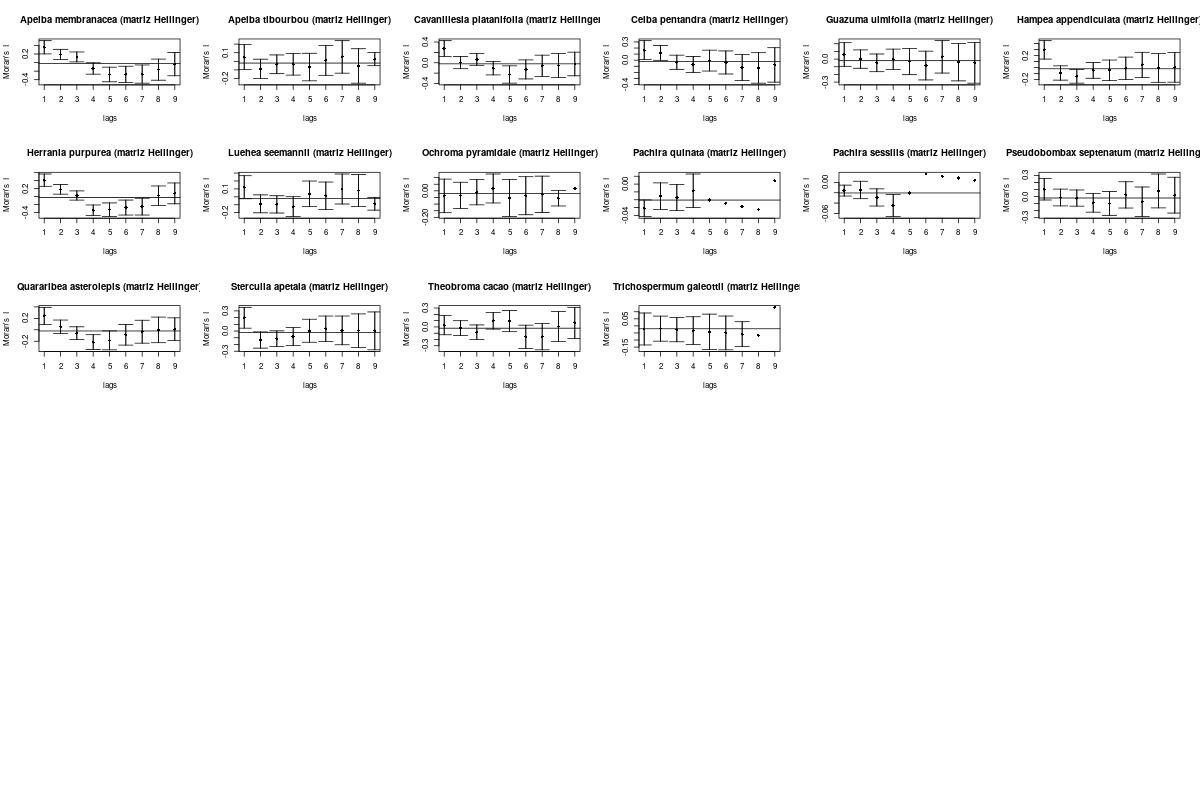
\includegraphics[width=0.50000\textwidth]{correlograma_matriz_de_comunidad_transformda.jpg}
\caption{Correlograma de matriz de comunidad transformada por especies
de plantas}
\end{figure}

\begin{figure}
\centering
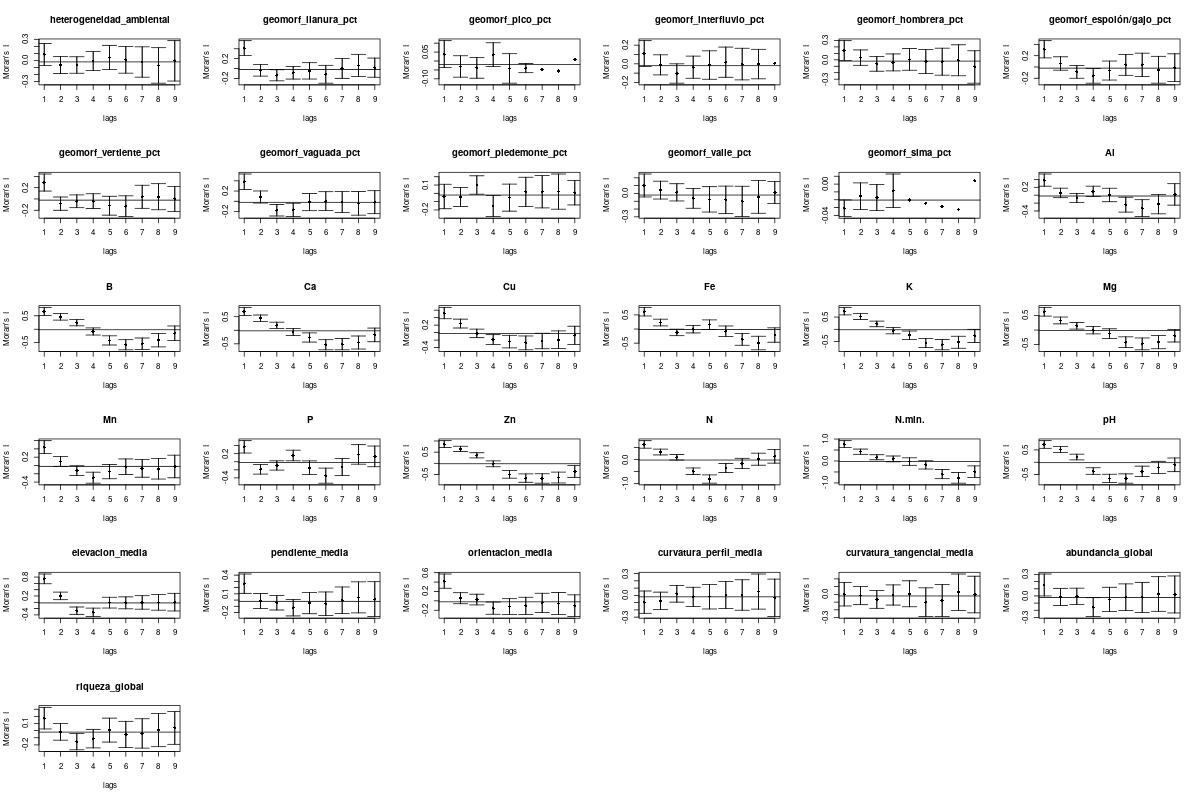
\includegraphics[width=0.50000\textwidth]{correlacion_matriz_comunidad_geomorofologicas_variables_suelo.jpg}
\caption{Correlación entre variables geomorfológicas y elementos del
suelo}
\end{figure}

\begin{figure}
\centering
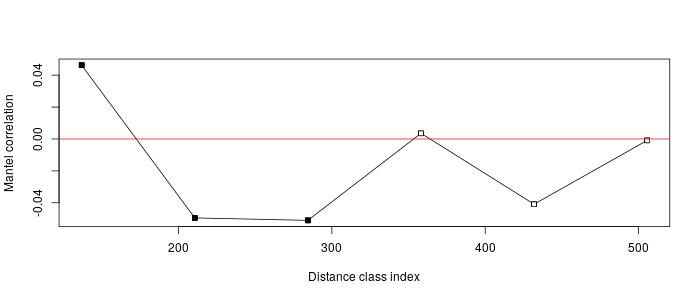
\includegraphics[width=0.50000\textwidth]{mi_fam_correlograma.jpg}
\caption{Correlograma de las diferentes especies de Malvaceae}
\end{figure}

El correlograma muestra que para el nivel de significancia 0.01 hay
autocorrelacion asi como para los 200 metros y para los otros ordenes
hay una autocorrelación espacial de este modo se observó una dependeica
espacial autocorrelación inducida

\begin{figure}
\centering
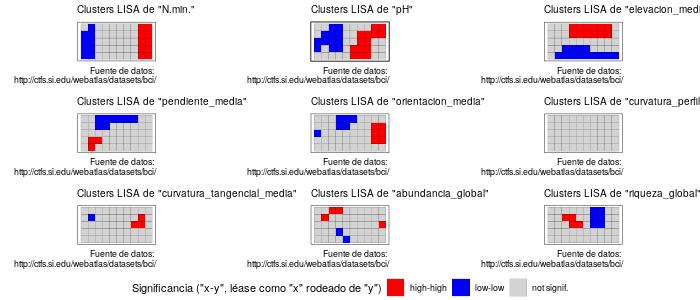
\includegraphics[width=0.50000\textwidth]{cluster_LISA.jpg}
\caption{Cluster LISA aplicado a variables ambientales}
\end{figure}

Los cuadros rojos es la autocorrelación espacial con valores altos y el
azul reprsenta una autocorrelación espacial con valores bajos Estos
clúster LISA muestran que el PH es la variable que mas esta
autocorrelacionada lo que quiere decir que ese lugar es muy acido y es
significativamente alto. La variable de elevación media esta al norte
donde BCI es mas elevada

\begin{figure}
\centering
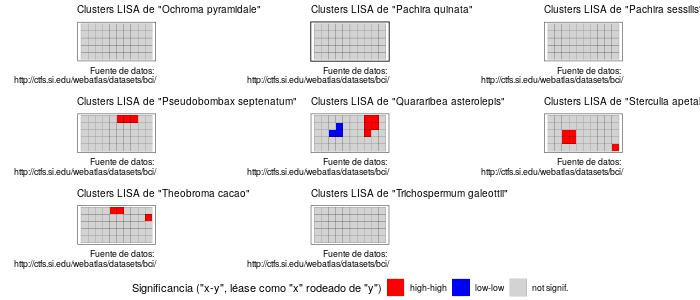
\includegraphics[width=0.50000\textwidth]{cluster_LISA_aplicado_especies_transformadas.jpg}
\caption{Cluster LISA aplicado especies transformadas}
\end{figure}

En este caso Quararibea asterolepis tiene valores abundancias grandes
rodeadas de abundancias grandes. Otras especies como Sterculia apetala,
Theobroma cacao y Pseudobombax septenatum muestraun un patrón similar
aunque en menor medida.

\section{Discusión}\label{discusiuxf3n}

El estudio presentó las diversas formas método de análisis de datos que
descomponga la varianza total de un sitio por especie.

\section{Agradecimientos}\label{agradecimientos}

\section{Información de soporte}\label{informaciuxf3n-de-soporte}

\ldots

\section{\texorpdfstring{\emph{Script}
reproducible}{Script reproducible}}\label{script-reproducible}

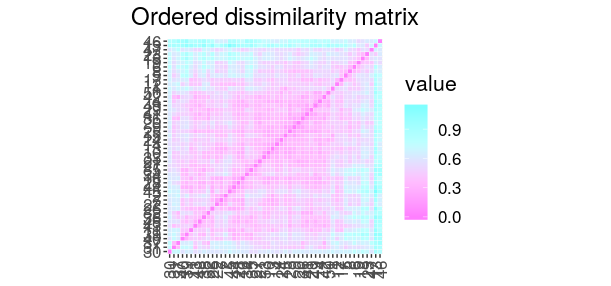
\includegraphics[width=0.50000\textwidth]{matriz_de_dismilaridad_mejorados.png}
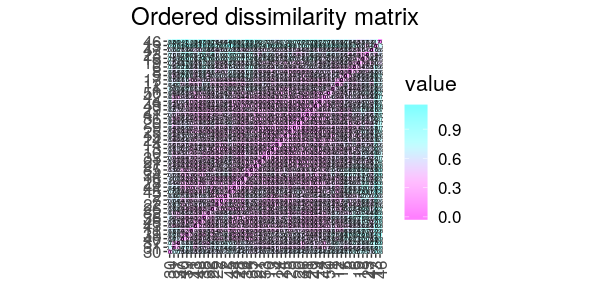
\includegraphics[width=0.50000\textwidth]{Matriz_disimilaridad_sobreimpresos.png}

\begin{figure}
\centering
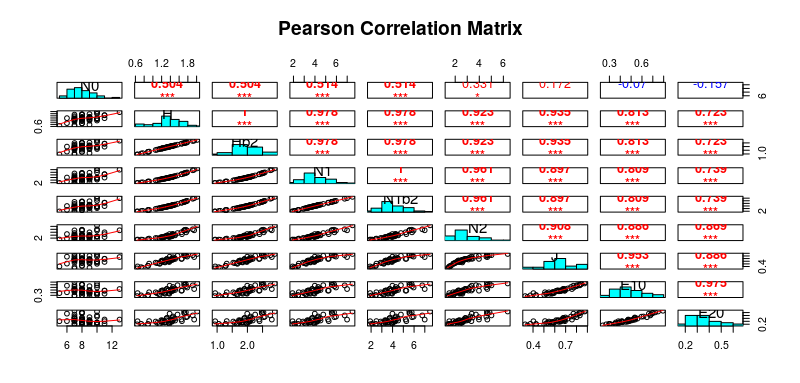
\includegraphics[width=0.50000\textwidth]{Indice_correlacion_Pearson.png}
\caption{Indice de correlaciónd e
pearsons\label{fig:matriz_disimilaridad}}
\end{figure}

\begin{figure}
\centering
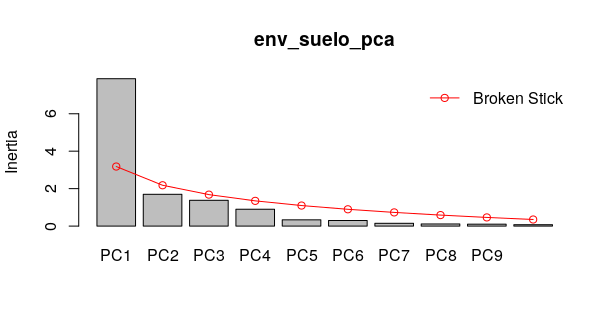
\includegraphics[width=0.50000\textwidth]{modelo_barra_quebrada.png}
\caption{Barra quebrada modelo}
\end{figure}

\begin{figure}
\centering
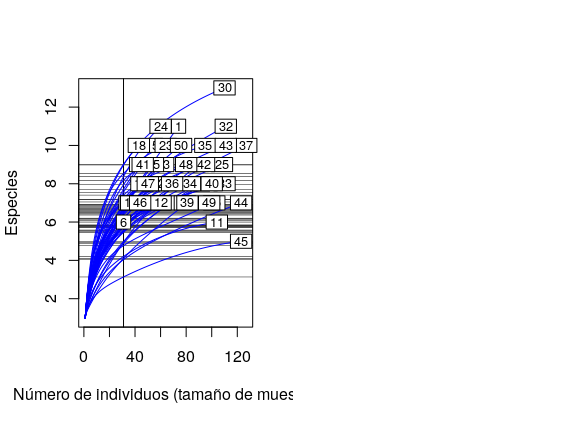
\includegraphics[width=0.50000\textwidth]{grafico_de_rarefaccion.png}
\caption{Gráfico de rarefacción}
\end{figure}

\begin{figure}
\centering
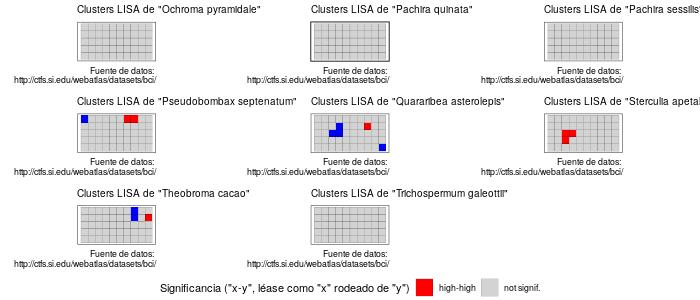
\includegraphics[width=0.50000\textwidth]{cluster_LISA_aplicado_especies_transformadas_sin_tendencia.jpg}
\caption{Cluster LISA aplicado a especies (sin tendencia)}
\end{figure}




\newpage
\singlespacing 
\end{document}
